\documentclass{standalone}
\usepackage{color}
\usepackage{tikz}
\usetikzlibrary{shapes,arrows,arrows.meta,fit,positioning}

\newcommand{\defaultwidth}{3cm}
\tikzset{
    auto, node distance = 1.1cm,
    stage/.style = { draw, thick, rectangle, align=center,
        text width = \defaultwidth, 
        font=\bfseries,
        rounded corners=2mm, 
        minimum width = \defaultwidth
    },
    note/.style = { draw, very thin, rectangle, dashed, align=center,
        node distance = 0.5cm,
        text width = \defaultwidth - 1cm, 
        font=\footnotesize,
        minimum width = \defaultwidth - 1cm
    },
    arrow/.style = { -latex, thick },
    arrow_text/.style = { align=center,
        pos = 0.5,
        font = \scriptsize
    }
}

\begin{document}
    \begin{tikzpicture}
        \node[stage] (0) at (0,0)
            {Initial\\conditions\\
            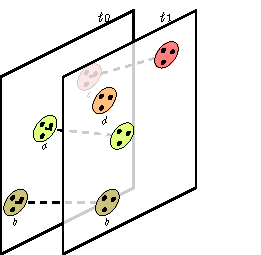
\includegraphics[width=\defaultwidth]{stage0}};
        \node[stage] (1) [below = 5mm of 0]
            {Getting\\ new disks\\
            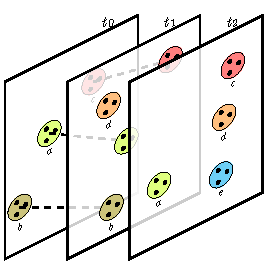
\includegraphics[width=\defaultwidth]{stage1}};
        \node[stage] (2) [right = 5mm of 1]
            {Joining disks \\
            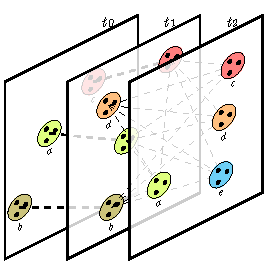
\includegraphics[width=\defaultwidth]{stage2}};
        \node[stage] (3) [right = 5mm of 2]
            {Reporting\\flocks \\
            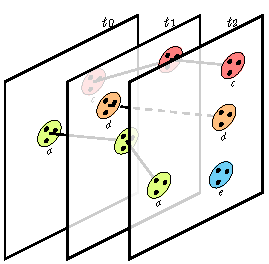
\includegraphics[width=\defaultwidth]{stage3}};
        \node[stage] (4) [right = 5mm of 3]
            {Updating\\flocks \\
            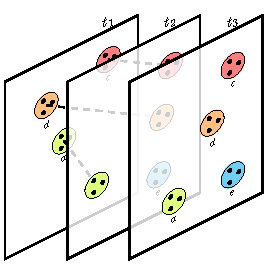
\includegraphics[width=\defaultwidth]{stage4}};

        \draw[arrow] (0) -- (1);
        \draw[arrow] (1) -- (2);
        \draw[arrow] (2) -- (3);
        \draw[arrow] (3) -- (4);

    \end{tikzpicture}
\end{document}
